\documentclass[letterpaper, 10pt, conference]{ieeeconf}
%DIF LATEXDIFF DIFFERENCE FILE
%DIF DEL ACC15.tex         Fri Sep 26 10:48:42 2014
%DIF ADD ACC15_Final.tex   Fri Sep 26 12:02:40 2014
\IEEEoverridecommandlockouts \overrideIEEEmargins
\usepackage{amsmath,amssymb,url}
\usepackage{graphicx,subfigure,tikz,graphicx}
\usepackage{color}
\usepackage{csquotes}


\newcommand{\argmax}{\operatornamewithlimits{argmax}}
\newcommand{\expm}{\ensuremath{\mathrm{expm}}}
\newcommand{\diag}{\mathop{\mathrm{diag}}\nolimits}
\newcommand{\norm}[1]{\ensuremath{\left\| #1 \right\|}}
\newcommand{\bracket}[1]{\ensuremath{\left[ #1 \right]}}
\newcommand{\braces}[1]{\ensuremath{\left\{ #1 \right\}}}
\newcommand{\parenth}[1]{\ensuremath{\left( #1 \right)}}
\newcommand{\pair}[1]{\ensuremath{\langle #1 \rangle}}
\newcommand{\met}[1]{\ensuremath{\langle\langle #1 \rangle\rangle}}
\newcommand{\refeqn}[1]{(\ref{eqn:#1})}
\newcommand{\reffig}[1]{Fig. \ref{fig:#1}}
\newcommand{\tr}[1]{\mathrm{tr}\ensuremath{\negthickspace\bracket{#1}}}
\newcommand{\trs}[1]{\mathrm{tr}\ensuremath{[#1]}}
\newcommand{\ave}[1]{\mathrm{E}\ensuremath{[#1]}}
\newcommand{\deriv}[2]{\ensuremath{\frac{\partial #1}{\partial #2}}}
\newcommand{\SO}{\ensuremath{\mathsf{SO(3)}}}
\newcommand{\T}{\ensuremath{\mathsf{T}}}
\renewcommand{\L}{\ensuremath{\mathsf{L}}}
\newcommand{\so}{\ensuremath{\mathfrak{so}(3)}}
\newcommand{\SE}{\ensuremath{\mathsf{SE(3)}}}
\newcommand{\se}{\ensuremath{\mathfrak{se}(3)}}
\renewcommand{\Re}{\ensuremath{\mathbb{R}}}
\newcommand{\aSE}[2]{\ensuremath{\begin{bmatrix}#1&#2\\0&1\end{bmatrix}}}
\newcommand{\ase}[2]{\ensuremath{\begin{bmatrix}#1&#2\\0&0\end{bmatrix}}}
\newcommand{\D}{\ensuremath{\mathbf{D}}}
\renewcommand{\d}{\ensuremath{\mathfrak{d}}}
\newcommand{\Sph}{\ensuremath{\mathsf{S}}}
\renewcommand{\S}{\Sph}
\newcommand{\J}{\ensuremath{\mathbf{J}}}
\newcommand{\Ad}{\ensuremath{\mathrm{Ad}}}
\newcommand{\intp}{\ensuremath{\mathbf{i}}}
\newcommand{\extd}{\ensuremath{\mathbf{d}}}
\newcommand{\hor}{\ensuremath{\mathrm{hor}}}
\newcommand{\ver}{\ensuremath{\mathrm{ver}}}
\newcommand{\dyn}{\ensuremath{\mathrm{dyn}}}
\newcommand{\geo}{\ensuremath{\mathrm{geo}}}
\newcommand{\Q}{\ensuremath{\mathsf{Q}}}
\newcommand{\G}{\ensuremath{\mathsf{G}}}
\newcommand{\g}{\ensuremath{\mathfrak{g}}}
\newcommand{\Hess}{\ensuremath{\mathrm{Hess}}}
\newcommand\circled[1]{%
  \tikz[baseline=(C.base)]\node[draw,circle,inner sep=0.5pt](C) {#1};\!
}


\title{\LARGE \bf
%Systematic Reduction of Uncertainty and Coalescence from JPDA Filtering
%Minimum Uncertainty JPDA Filtering and Advancements on Avoiding Coalescence
Minimum Uncertainty JPDA Filter and Coalescence Avoidance}
\author{Evan Kaufman, Thomas Alan Lovell, and Taeyoung Lee$^*$
 \thanks{Evan Kaufman and Taeyoung Lee are with Department of Aerospace Engineering, George Washington University, Washington, DC. Email: {\tt\footnotesize \{evankaufman, tylee\}@gwu.edu }}
\thanks{Thomas Alan Lovell is a Research Aerospace Engineer at the Space Vehicles Directorate, Air Force Research Lab (AFRL), Albuquerque, NM. Email: {\tt\footnotesize afrl.rvsv@kirtland.af.mil }}
\thanks{$^*$This research has been supported in part by NSF under the grants CMMI-1243000 (transferred from 1029551), CMMI-1335008, and CNS-1337722.}}


%\newcommand{\EditTL}[1]{{\color{blue}\protect #1}}
%\renewcommand{\EditTL}[1]{{\protect #1}}

\newtheorem{definition}{Definition}
\newtheorem{lem}{Lemma}
\newtheorem{prop}{Proposition}
\newtheorem{remark}{Remark}


%\usepackage{ulem}
%DIF PREAMBLE EXTENSION ADDED BY LATEXDIFF
%DIF UNDERLINE PREAMBLE %DIF PREAMBLE
\RequirePackage[normalem]{ulem} %DIF PREAMBLE
\RequirePackage{color}\definecolor{RED}{rgb}{1,0,0}\definecolor{BLUE}{rgb}{0,0,1} %DIF PREAMBLE
\providecommand{\DIFadd}[1]{{\protect\color{blue}\uwave{#1}}} %DIF PREAMBLE
\providecommand{\DIFdel}[1]{{\protect\color{red}\sout{#1}}}                      %DIF PREAMBLE
%DIF SAFE PREAMBLE %DIF PREAMBLE
\providecommand{\DIFaddbegin}{} %DIF PREAMBLE
\providecommand{\DIFaddend}{} %DIF PREAMBLE
\providecommand{\DIFdelbegin}{} %DIF PREAMBLE
\providecommand{\DIFdelend}{} %DIF PREAMBLE
%DIF FLOATSAFE PREAMBLE %DIF PREAMBLE
\providecommand{\DIFaddFL}[1]{\DIFadd{#1}} %DIF PREAMBLE
\providecommand{\DIFdelFL}[1]{\DIFdel{#1}} %DIF PREAMBLE
\providecommand{\DIFaddbeginFL}{} %DIF PREAMBLE
\providecommand{\DIFaddendFL}{} %DIF PREAMBLE
\providecommand{\DIFdelbeginFL}{} %DIF PREAMBLE
\providecommand{\DIFdelendFL}{} %DIF PREAMBLE
%DIF END PREAMBLE EXTENSION ADDED BY LATEXDIFF

\begin{document}
\allowdisplaybreaks


\maketitle \thispagestyle{empty} \pagestyle{empty}

\begin{abstract}
This paper deals with an estimation problem where a known number of objects in close proximity are observed but the measurement origins are uncertain.
It is well known that the joint probabilistic data association filter (JPDAF) is effective in handling uncertain measurement originations with clutter, but the algorithm suffers it two ways addressed in this paper: first, the JPDAF directly adopts the gain of Kalman filters that does not minimize the posterior uncertainty of the JPDAF.
In this paper, an analytic solution for an optimal gain is derived that minimizes this uncertainty, and the corresponding filter is referred to as the minimum uncertainty JPDAF (MUJPDAF).
Second, the JPDAF is well-known to cause coalescence of estimates when objects are in close proximity.
This paper introduces a new variation of JPDAF, referred to as the coalescence-avoiding optimal JPDAF (C-JPDAF), which removes coalescence by minimizing a weighted sum of the posterior uncertainty and a measure of similarity between estimated probability densities.
This approach takes a simpler structure than other coalescence avoiding approaches based on pruning, while exhibiting excellent filtering performance for objects in close proximity with close or crossing tracks. Both algorithms are illustrated by numerical examples of satellites in close proximity orbiting around the Earth.
\end{abstract}

%_______________________________________________%

\section{Introduction}

Data association has been extensively studied with various applications in estimation when measurements are not necessarily originating from a single object.
We consider applications wherein multiple objects of interest enter the field of view of a sensor; however, the measurement origins are unknown.
To properly track these objects, we require estimation techniques that associate objects with measurements.
When the objects are in very close proximity, the association uncertainties grow, and an effective algorithm is necessary to maintain \DIFdelbegin \DIFdel{close }\DIFdelend \DIFaddbegin \DIFadd{accurate }\DIFaddend estimations of the objects~\cite{KauLovLee14}.

A variety of data association techniques are considered for close-proximity trajectories with varying performance.
Multiple hypothesis tracking (MHT) and probability hypothesis density (PHD) techniques involve a high computational load, especially when objects are in close proximity, making real-time implementation more difficult~\cite{MHT1},~\cite{PHD1},~\cite{PHD2}.
Many other techniques are based on the Kalman filter (KF) or extended KF (EKF), which provide a framework for recursive data association techniques for easier real-time implementation.
There are two popular strategies among recursive approaches, namely \emph{hard decisions} and \emph{soft decisions}~\cite{JPDAF1}.
A hard decision is when estimates are fully associated with measurements according to some metric between the estimates and the measurements.
For example, a common heuristic approach is known as the nearest neighbor filter (NNF), which uses the Mahalanobis distance between each measurement and the predicted measurements of each potential object that may be associated with that measurement.
The measurement with the smallest Mahalanobis distance is considered as the correct one~\cite{NN2}.
However, when estimates are in close proximity, there is a high likelihood of making incorrect associations, which may be detrimental to the estimated states, so this technique is avoided in the analysis of this paper.

Alternatively with a soft decision technique such as the \DIFdelbegin \DIFdel{JPDAF}\DIFdelend \DIFaddbegin \DIFadd{joint probabilistic data association filter (JPDAF)}\DIFaddend , measurements are shared among the estimates. With the JPDAF, the likelihoods of association between measurements and estimates serve as weighting factors inside the measurement update portion of the filtering~\cite{JPDAF1},~\cite{TrackDataAssoc}.
The JPDAF is particularly advantageous in multi-object scenarios because when objects share measurements, the soft decisions prevent loss of information, which occurs with hard decision approaches.
%The a posteriori uncertainties of the estimates are changed because of an additional term representing the spread in the innovations; the Kalman gain serves as a close estimate to an optimal gain in the sense that in nearly minimizes this a posteriori gain as derived by the linearized equations of the JPDAF.
The JPDAF is based on the Kalman gain, which \DIFdelbegin \DIFdel{minimizes }\DIFdelend \DIFaddbegin \DIFadd{reduce }\DIFaddend the posterior uncertainty of individual tracks.
However, the Kalman gain is not guaranteed to \emph{exactly} minimize the posterior uncertainties \DIFaddbegin \DIFadd{for data association }\DIFaddend of the JPDAF.
%The unnecessarily large uncertainty of the suboptimal Kalman gain serves as motivation to derive an optimal gain that minimizes the a posteriori uncertainty of the linearized JPDAF equations.
\DIFaddbegin 

\DIFaddend In this paper, we derive the optimal estimation gain that minimizes the magnitude of the posterior covariance matrix, and the resulting minimum uncertainty JPDAF is referred to as the MUJPDAF.

The second part of this paper deals with the cases when neighboring objects share measurements, where the estimates are subject to coalescence.
Most techniques to avoid track coalescence involve pruning the tracks, or designing a set of rules that limit the possible outcomes to likely scenarios. These rules typically involve exact nearest neighbor probabilistic data association (ENNPDA), which applies a strong decision to the most likely associated estimate. Pruning algorithms incorporate the ENNPDA algorithm because  estimates do not share measurements, making it insensitive to track coalescence~\cite{Coal1}.
For example in~\cite{Fitzgerald}, the algorithm involves a set of rules to prune the tracks that share measurements.
The algorithm considers the possible combinations of estimate-to-measurement associations over a time window and applies a logic that assigns estimates to likely scenarios; a set of possible scenarios are considered and lower likelihood scenarios are deleted~\cite{Coal_d},~\cite{Coal_e},~\cite{Coal_c}.
However, track pruning assumes that low likelihood association scenarios are incorrect, which is not necessarily true.
Furthermore, removing the weighting scheme of the JPDAF causes the estimates to lose information.

Therefore, we propose a new coalescence-avoiding optimal JPDAF referred to as the C-JPDAF, which is a systematic approach to remove coalescence by minimizing the weighted sum of the uncertainty and a similarity index between estimates~\cite{KauLovLee14}.
The prior \DIFdelbegin \DIFdel{research }\DIFdelend \DIFaddbegin \DIFadd{work }\DIFaddend covers the concept in simple cases, such that only two estimates are considered with a single measurement at each time step, making the algorithm infeasible in many realistic applications.
Therefore, we generalize the algorithm to handle any number of objects and measurements, as well as missed detections and measurements originating from extraneous clutter.
%Therefore we mature the algorithm to have the same assumptions as the JPDAF.
%Most importantly, there may be a variable number of measurements for a known number of estimates such that missed detections and false alarms are no longer an issue.

The paper is organized as follows: the data association filtering problem is formally presented in Section \ref{ProbDef}.
The posterior uncertainty according to the JPDAF equations is minimized to derive the MUJPDAF, which is compared with the conventional JPDAF equations in Section \ref{MUJPDAF}.
An optimal gain that minimizes a weighted cost of uncertainty and similarity in a general sense is derived in Section \ref{C-JPDAF}.
Numerical examples show how each of these algorithms can be advantageous and how they compare to each other in Section \ref{NumRes}, followed by conclusions.

\section{Data Association Filtering Problem Formulation}
\label{ProbDef}

 This section describes the dynamics of objects and the measurement model considered in this paper and a filtering problem is formulated. 

\subsection{Dynamics of Objects and Measurements}

%
% Linearized equations of motion: assumed known
% Assume the Gaussian noise model and define unknown random variables $w$ (process noise) and $v$ (measurement noise)
% Initial conditions are assumed known, define $\hat x_{i,0}$, $P^+_{i,0}$

%Define the set of all objects $I=\{1,2,...,t\}$ such that the object index $i\in I$ where the total number of objects $t$ is assumed known.
Consider $n_t$ objects indexed by $i\in I=\{1,2,...,n_t\}$, where $n_t$ is assumed known.
The dynamics of the $i$-th object are modeled as a linear stochastic discrete-time system described by
\begin{align}
x_{i_{k}} & = F_{i_{k-1}} x_{i_{k-1}} + w_{i_{k}},\label{eqn:xkp}\\
z_{i_k} & = H_{i_k} x_{i_k} + v_{i_k},
\end{align}
where $x_{i_k}\in\Re^n$ is the state vector, $z_{i_k}\in\Re^m$ is the output vector, and  the matrices $F_{i_{k-1}}\in\Re^{n\times n}$ and $H_{i_k}\in\Re^{m\times n}$ describe system dynamics and outputs.
The process noise and the measurement noise are denoted by $w_{i_k}\in\Re^n$ and $v_{i_k}\in\Re^m$, respectively, where they are assumed to be zero-mean, mutually independent white, Gaussian noise sequences with known covariance matrices $Q_{i_k}\in\Re^{n\times n}$ and $R_{i_k}\in\Re^{m\times m}$, respectively, i.e.,
\begin{align}
w_{i_k} \sim \mathcal{N}[0,Q_{i_k}],\quad
v_{i_k} \sim \mathcal{N}[0,R_{i_k}],
\end{align}
where $\mathcal{N}[\mu,\sigma]$ denotes the Gaussian distribution with mean $\mu$ and standard deviation $\sigma$.


The initial states are also assumed to be mutually independent with noise. They are Gaussian with known mean values and covariance matrices:
\begin{align}
x_{i_0} \sim \mathcal{N}[\bar x_{i_0}, P_{i_0}],\label{eqn:xi0}
\end{align}
where $\bar x_{i_0}\in\Re^n$ and $P_{i_0}\in\Re^{n\times n}$. 

%To demonstrate the main idea of the proposed data association filter concisely, it is assumed that there are two objects, i.e., $i\in\{1,2\}$. But, the results of this paper are readily generalized to arbitrary number of systems provided the number of objects is known.

\subsection{Measurement Origination Model}
\label{DAP}

% Likelihoods of association are calculated from the innovations and innovation covariances only
% Two techniques are used to obtain the likelihoods of association, both of which may be applied to the JPDAF, MUJPDAF, and C-JPDAF
	% "Cheap JPDAF": inexpensive calculation, present the four equations and two references
	% True likelihood of association: infeasible for many real-time applications, calculated in the appendix

%Define the set $J=\{1,2,...,r\}$ such that the measurement index $j\in J$ where $r$ is a variable number of measurement returns such that $r\geq1$.
Suppose that there are $n_r$ measurements indexed by $j\in J=\{1,2,...,n_r\}$.
Let $\beta_{ij}$ be the probability that the $i$-th system is associated with measurement $j$.
Two techniques may be applied to solve for every $\beta_{ij}$, both of which require the innovation and its covariance (defined later) and information on detection probabilities, which are assumed known.
The first technique is applied in the standard JPDAF that calculates the true association probabilities from~\cite[Eq. 9.(45-46)]{TrackDataAssoc}.
However, the computation required with a standard JPDAF is inconsistent with the capabilities of the computational resources to account for an arbitrary number of objects to be tracked~\cite{Bar1990}.

A modified version of the JPDA, commonly known as the ``Cheap JPDA'', provides a simpler approximation of the likelihood $\beta_{ij}$.
The equations below are adopted from~\cite[Eq. 1.(1-2)]{Bar1990}.
Let $G_{ij}$ be a variable which takes a very similar form as the Gaussian probability density function
\begin{align}
G_{ij}=\frac1{\sqrt{\det{S_{i}}}}\exp{\{-\frac12e_{ij}^TS_{i}^{-1}e_{ij}\}},
\end{align}
where $e_{ij}$ is the innovation and $S_{i}$ is the a priori innovation covariance, defined later in \refeqn{eij} and \refeqn{S}, respectively.
This is used to calculate intermediate variables $\mathcal{S}_{ti}$ and $\mathcal{S}_{ri}$
\begin{align}
\mathcal{S}_{ti}=\sum\limits_{j\in J}G_{ij}, 
\quad 
\mathcal{S}_{ri}=\sum\limits_{i\in I}G_{ij}.
\end{align}
The probability that the $i$-th system is associated with the $j$-th measurement is
\begin{align}
\beta_{ij}=\frac{G_{ij}}{\mathcal{S}_{ti}+\mathcal{S}_{ri}-G_{ij}+B}, 
\end{align}
where $B$ is a correction factor to account for a non-unity probability of detection.

\section{Minimum Uncertainty Probabilistic Data Association Filter (MUJPDAF)}
\label{MUJPDAF}

In this section we derive the MUJPDAF that minimizes the posterior estimate uncertainties.
Differences between the JPDAF and MUJPDAF occur in the measurement update where the gain is derived, which changes the posterior covariance equation.

\subsection{Flow Update}

During the flow update, \DIFdelbegin \DIFdel{the }\DIFdelend a priori (denoted with \DIFaddbegin \DIFadd{the }\DIFaddend superscript $-$) \DIFdelbegin \DIFdel{estimated state }\DIFdelend \DIFaddbegin \DIFadd{estimate }\DIFaddend $\hat x_{i_k}^-$ is found with \refeqn{xkp} and its a priori covariance $P_{i_k}^-$ is calculated from the last posterior (denoted with superscript $+$) covariance $P_{i_{k-1}}^+$ for all $i$ as
\begin{gather}
%\hat x_{i_{k}}^- = f(\hat x_{i_{k-1}}^+),\\
P_{i_{k}}^- = F_{i_{k-1}} P_{i_{k-1}}^+ F_{i_{k-1}}^T + Q_{i_{k}}.
\end{gather}
These equations are applied between measurements to provide predictions of the states and their uncertainties.
% Equations for a priori state estimates and covariances

\subsection{Measurement Update}

The measurements serve to update the state estimates. Because all equations in this section take place at the $k$ time step, this subscript is removed from the equations. For a given measurement $z_j$, its measurement residual or innovation for the $i$-th object is given by
\begin{align}
e_{ij} = z_j - \hat z_i,\label{eqn:eij}
\end{align}
where $\hat z_i$ is the predicted measurement from $\hat x_{i}^-$ and a known measurement matrix $H_i$ such that
\begin{align}
\hat z_i = H_i\hat x_{i}^-.
\end{align}
%where the true measurement is expected to be
%\begin{align}
%z_i=h(x_i)+v_i, \quad H_i=\frac{\partial h}{\partial x}\bigg|_{x=\hat x_{i}^- }.
%\end{align}
Given the uncertainty of the measurements represented with covariance $R_i$, the \DIFdelbegin \DIFdel{a }\DIFdelend priori innovation covariance $S_{i}$ is
\begin{align}
S_{i}=H_{i}P_{i}^{-}H_{i}^T+R_{i}.\label{eqn:S}
\end{align}

The weighted sum of all innovations associated with the object $i$ is defined as ${\bf{e}}_{i}={\sum\limits_{j\in J} \beta_{ij}e_{ij}}$.
The resulting posterior estimate of the state is given by
%~\cite[Eq. 6-(25-26)]{TrackDataAssoc}
\begin{align}
\hat x^+_{i}=&\ \hat x^-_{i}+K_{i}{\bf{e}}_{i}.\label{eqn:KalEst}
\end{align}
The conventional JPDAF defines $K_i$ from the gain of the Kalman filter, given by $K_i=P^-_iH_i^TS_i^{-1}$, based on an incorrect assumption that the Kalman gain is always optimal for data association with the JPDAF.
%%____________________________________BEGIN NEW SECTION __________________________________%
%
%From \refeqn{eij} and \refeqn{KalEst}, $\hat x^+_{i}$ may be rewritten as
%\begin{align}
%\hat x_i^+&=\hat x^-+K_i\sum\limits_{j\in J}\beta_{ij}(z_j-H_i\hat x_i^-),\nonumber
%\\
%&=\left(I-(1-\beta_{0,i})K_iH_i\right)\hat x_i^-+K_i\sum\limits_{j\in J}\beta_{ij}z_j.\label{eqn:xhatpDEF}
%\end{align}
%Because $z_i=H_ix_i+v$, the posterior state error is
%\begin{align}
%\tilde x_i^+&=\hat x_i^+-x_i,\label{eqn:xperr}
%\\
%&=\left(I-(1-\beta_{0,i})K_iH_i\right)\hat x^-+K_i\sum\limits_{j\in J}\beta_{ij}z_j-
%\end{align}
%
%The definition of the posterior covariance matrix $P^+_i$ is
%\begin{align}
%P^+_i=\mathrm{E}[\tilde x^+\tilde x^{+T}],
%\end{align}
%
%In this paper, we find $K_i$ to minimize the posterior uncertainty of the state estimate.
%The optimal gain $K_i$ is derived below in the sense that the posterior uncertainties are minimized with respect to the generalized equations of the JPDAF.
%%Of course, the estimator cannot be optimal if the system is nonlinear, because the linearized equations to not fully represent the dynamics of a nonlinear system.
%
%Let the probability that object $i$ is not associated with any measurement be $\beta_{0,i}=1-{\sum\limits_{j} \beta_{ij}}$.
%The resulting posterior covariance can be written as
%%~\cite[Eq. D-32 and D-33]{TrackDataAssoc}
%\begin{align}
%\label{eqn:JPDAFCov}
%P^+_{i}=&\ \beta_{0,i}P^-_{i}+(1-\beta_{0,i})P_i^c+\tilde P,
%\end{align}
%where $\tilde P\in\Re^{n\times n}$ is
%\begin{align}
%\tilde P=&\ K_i\left({\sum\limits_{j} \beta_{ij}e_{ij}e_{ij}^T-{\bf{e}}_{i}}{\bf{e}}_{i}^T\right)K_{i}^T,\label{eqn:tildeP}
%\end{align}
%and $P_i^c$ corresponds to the posterior covariance of object $i$ if only a single measurement serves to update this track~\cite{TrackDataAssoc}, and it can be written as
%%We can define $P_i^c$ without any assumptions on $K_i$ (i.e. $K_i$ is not necessarily the Kalman gain, so the well-known Kalman covariance update equations are not valid here) as~\cite[Eq. 4.2-12]{OptEst1}
%\begin{align}
%P^c_i=&\ (I-K_iH_i)P^-_i(I-K_iH_i)^T+K_iR_iK_i^T,\nonumber
%\\
%=&\ P^-_i-(K_iH_iP^-_i+P^-_iH_i^TK_i^T)\nonumber
%\\
%&\ +K_i(H_iP^-_iH_i^T+R_i)K_i^T,
%\label{eqn:GenCov}
%\end{align}
%(see~\cite{OptEst1}).
%Substituting \refeqn{tildeP} and \refeqn{GenCov} into \refeqn{JPDAFCov} and rearranging,
%\begin{align}
%P^+_{i}=&\ \beta_{0,i}P^-_{i}+(1-\beta_{0,i})[P^-_i-(K_iH_iP^-_i+P^-_iH_i^TK_i^T)\nonumber
%\\
%&\ +K_i(H_iP^-_iH_i^T+R_i)K_i^T]\nonumber
%\\
%&\ +K_i\left({\sum\limits_{j} \beta_{ij}e_{ij}e_{ij}^T-{\bf{e}}_{i}}{\bf{e}}_{i}^T\right)K_{i}^T,\nonumber
%\\
%=&\ P^-_{i}-(1-\beta_{0,i})(K_iH_iP^-_i+P^-_iH_i^TK_i^T)\nonumber
%\\
%&\ +K_i\left((1-\beta_{0,i})S_i+{\sum\limits_{j} \beta_{ij}e_{ij}e_{ij}^T-{\bf{e}}_{i}}{\bf{e}}_{i}^T\right)K_i^T,\nonumber
%\\
%=&\ P^-_{i}-(1-\beta_{0,i})(K_iH_iP^-_i+P^-_iH_i^TK_i^T)\nonumber
%\\
%&\ +K_iE_iK_i^T,\label{eqn:CovExpanded}
%\end{align}
%where the symmetric matrix $E_i=E_i^T\in\Re^{m\times m}$, defined as
%\begin{align}
%E_i=&\ (1-\beta_{0,i})S_i+{\sum\limits_{j} \beta_{ij}e_{ij}e_{ij}^T-{\bf{e}}_{i}}{\bf{e}}_{i}^T.
%\end{align}
%Note that $E_i$ is independent of $K_i$ and is invertible when $\beta_{0,i}\neq1$ since $S_i$ is positive-definite and
%%may be calculated without knowledge of the gain matrix $K_i$, and is invertible because $P^-_i$ and $R_i$ are positive-definite and
%$(\beta_{ij}e_{ij}e_{ij}^T-{\bf{e}}_{i}{\bf{e}}_{i}^T)$ is positive-semidefinite, as shown in the Appendix A. 
%The case when $\beta_{0,i}=1$ corresponds with the $i$-th object \emph{not} being measured with full certainty.
%This case is analyzed in Appendix B.
%
%As with the Kalman filter, we choose the estimation gain to minimize the magnitude of the posterior covariance measured by $\tr{P_i^+}$.
%It requires that
%\begin{align}
%0&=\frac{\partial\tr{P^+_i}}{\partial K_i},\nonumber
%\\
%&=-2(1-\beta_{0,i})\frac{\partial\tr{K_iH_iP^-_i}}{\partial K_i}+\frac{\partial\tr{K_iE_iK_i^T}}{\partial K_i},\nonumber
%\\
%&=-2(1-\beta_{0,i})P^-_iH_i^T+2K_iE_i.\label{eqn:Uncertainty0}
%\end{align}
%Therefore the optimal gain is given by
%\begin{align}
%K_i&=(1-\beta_{0,i})P^-_iH_i^TE_i^{-1}.\label{eqn:GainK}
%\end{align}
%
%Finally, \refeqn{GainK} is substituted into \refeqn{CovExpanded} to obtain
%\begin{align}
%%\begin{split}
%%P^+_{i}=&P^-_{i}-(1-\beta_{0,i})^2(P^-_iH_i^TE_i^{-1}H_iP^-_i
%%\\
%%&+P^-_iH_i^TE_i^{-1}H_iP^-_i
%%-P^-_iH_i^TE_i^{-1}E_iE_i^{-1}H_iP^-_i)
%%\end{split}
%%\\
%P^+_{i}=&P^-_{i}-(1-\beta_{0,i})^2P^-_iH_i^TE_i^{-1}H_iP^-_i,
%\end{align}
%which may be simplified in two ways
%\begin{align}
%P^+_{i}=&P^-_{i}-K_iE_iK_i^T, \quad \mbox{or equivalently}\label{eqn:JPDAFPostCovSymmetricUpdate}
%\\
%P^+_{i}=&\left(I-(1-\beta_{0,i})K_iH_i\right)P^-_i.\label{eqn:JPDAFPostCovSimpleUpdate}
%\end{align}
%The proposed gain is compared with the Kalman gain explicitly in Appendix C.
%In short, the differences between the MUJPDAF and the conventional JPDAF are shown in \refeqn{GainK} and \refeqn{JPDAFPostCovSymmetricUpdate} or \refeqn{JPDAFPostCovSimpleUpdate}.
\DIFdelbegin \DIFdel{The }\DIFdelend \DIFaddbegin \DIFadd{Here we derive the }\DIFaddend optimal gain $K_i$ \DIFdelbegin \DIFdel{is derived below in the sense }\DIFdelend \DIFaddbegin \DIFadd{such }\DIFaddend that the posterior uncertainties are minimized with respect to the generalized equations of the JPDAF.
%Of course, the estimator cannot be optimal if the system is nonlinear, because the linearized equations to not fully represent the dynamics of a nonlinear system.

Let the probability that object $i$ is not associated with any measurement be $\beta_{0,i}=1-{\sum\limits_{j} \beta_{ij}}$.
The resulting posterior covariance can be written as
%~\cite[Eq. D-32 and D-33]{TrackDataAssoc}
\begin{align}
\label{eqn:JPDAFCov}
P^+_{i}=&\ \beta_{0,i}P^-_{i}+(1-\beta_{0,i})P_i^c+\tilde P,
\end{align}
where $\tilde P\in\Re^{n\times n}$ is
\begin{align}
\tilde P=&\ K_i\DIFdelbegin %DIFDELCMD < \left({%%%
\DIFdel{\sum}%DIFDELCMD < \limits%%%
\DIFdel{_{j} \beta_{ij}e_{ij}e_{ij}^T-}%DIFDELCMD < {\bf{e}}%%%
\DIFdel{_{i}}%DIFDELCMD < }{\bf{e}}%%%
\DIFdel{_{i}^T}%DIFDELCMD < \right)%%%
\DIFdelend \DIFaddbegin \parenth{{\sum\limits_{j} \beta_{ij}e_{ij}e_{ij}^T-{\bf{e}}_{i}}{\bf{e}}_{i}^T}\DIFaddend K_{i}^T,\label{eqn:tildeP}
\end{align}
and $P_i^c$ corresponds to the posterior covariance of object $i$ if only a single measurement serves to update this track~\cite{TrackDataAssoc}, and it can be written as
%We can define $P_i^c$ without any assumptions on $K_i$ (i.e. $K_i$ is not necessarily the Kalman gain, so the well-known Kalman covariance update equations are not valid here) as~\cite[Eq. 4.2-12]{OptEst1}
\begin{align}
P^c_i=&\ (I-K_iH_i)P^-_i(I-K_iH_i)^T+K_iR_iK_i^T,\nonumber
\\
=&\ P^-_i-(K_iH_iP^-_i+P^-_iH_i^TK_i^T)\nonumber
\\
&\ +K_i(H_iP^-_iH_i^T+R_i)K_i^T,
\label{eqn:GenCov}
\end{align}
(see~\cite{OptEst1}).
Substituting \refeqn{tildeP} and \refeqn{GenCov} into \refeqn{JPDAFCov} and rearranging,
\begin{align}
P^+_{i}=&\ \beta_{0,i}P^-_{i}+(1-\beta_{0,i})[P^-_i-(K_iH_iP^-_i+P^-_iH_i^TK_i^T)\nonumber
\\
&\ +K_i(H_iP^-_iH_i^T+R_i)K_i^T]\nonumber
\\
&\ +K_i\left({\sum\limits_{j} \beta_{ij}e_{ij}e_{ij}^T-{\bf{e}}_{i}}{\bf{e}}_{i}^T\right)K_{i}^T,\nonumber
\\
=&\ P^-_{i}-(1-\beta_{0,i})(K_iH_iP^-_i+P^-_iH_i^TK_i^T)\nonumber
\\
&\ +K_i\left((1-\beta_{0,i})S_i+{\sum\limits_{j} \beta_{ij}e_{ij}e_{ij}^T-{\bf{e}}_{i}}{\bf{e}}_{i}^T\right)K_i^T,\nonumber
\\
=&\ P^-_{i}-(1-\beta_{0,i})(K_iH_iP^-_i+P^-_iH_i^TK_i^T)\nonumber
\\
&\ +K_iE_iK_i^T,\label{eqn:CovExpanded}
\end{align}
where the symmetric matrix $E_i=E_i^T\in\Re^{m\times m}$, defined as
\begin{align}
E_i=&\ (1-\beta_{0,i})S_i+{\sum\limits_{j} \beta_{ij}e_{ij}e_{ij}^T-{\bf{e}}_{i}}{\bf{e}}_{i}^T.
\end{align}
Note that $E_i$ is independent of $K_i$ and is invertible when $\beta_{0,i}\neq1$ since $S_i$ is positive-definite and
%may be calculated without knowledge of the gain matrix $K_i$, and is invertible because $P^-_i$ and $R_i$ are positive-definite and
$(\beta_{ij}e_{ij}e_{ij}^T-{\bf{e}}_{i}{\bf{e}}_{i}^T)$ is positive-semidefinite, as shown in the Appendix A. 
The case when $\beta_{0,i}=1$ corresponds with the $i$-th object \emph{not} being measured with full certainty.
This case is analyzed in Appendix B.

As with the Kalman filter, we choose the estimation gain to minimize the magnitude of the posterior covariance measured by $\tr{P_i^+}$.
It requires that
%The only case where $E_i$ is not invertible is when $\beta_{0,i}=1$, or when there is full confidence that a particular object is not observed by any measurement.
%This is evaluated in the appendix to show that this case does not yield an infinite limit of the gain matrix derived below.
%
%The goal of the choosing $K_i$ is to minimize the uncertainty of the object state estimate.
%With a Kalman filter, this goal is accomplished by minimizing $\tr{P^+_i}$ with respect to $K_i$ for a single track and measurement; the same approach may be applied to the JPDAF, except the a posteriori covariance equation has changed, so $K_i$ is subject to change as well:
\begin{align}
0&=\frac{\partial\tr{P^+_i}}{\partial K_i},\nonumber
\\
&=-2(1-\beta_{0,i})\frac{\partial\tr{K_iH_iP^-_i}}{\partial K_i}+\frac{\partial\tr{K_iE_iK_i^T}}{\partial K_i},\nonumber
\\
&=-2(1-\beta_{0,i})P^-_iH_i^T+2K_iE_i.\label{eqn:Uncertainty0}
\end{align}
Therefore the optimal gain is given by
\begin{align}
K_i&=(1-\beta_{0,i})P^-_iH_i^TE_i^{-1}.\label{eqn:GainK}
\end{align}

Finally, \refeqn{GainK} is substituted into \refeqn{CovExpanded} to obtain
\begin{align}
%\begin{split}
%P^+_{i}=&P^-_{i}-(1-\beta_{0,i})^2(P^-_iH_i^TE_i^{-1}H_iP^-_i
%\\
%&+P^-_iH_i^TE_i^{-1}H_iP^-_i
%-P^-_iH_i^TE_i^{-1}E_iE_i^{-1}H_iP^-_i)
%\end{split}
%\\
P^+_{i}=&P^-_{i}-(1-\beta_{0,i})^2P^-_iH_i^TE_i^{-1}H_iP^-_i,
\end{align}
which may be simplified in two ways
\begin{align}
P^+_{i}=&P^-_{i}-K_iE_iK_i^T, \quad \mbox{or equivalently}\label{eqn:JPDAFPostCovSymmetricUpdate}
\\
P^+_{i}=&\left(I-(1-\beta_{0,i})K_iH_i\right)P^-_i.\label{eqn:JPDAFPostCovSimpleUpdate}
\end{align}
The proposed gain is compared with the Kalman gain explicitly in Appendix C.
In short, the differences between the MUJPDAF and the conventional JPDAF are shown in \refeqn{GainK} and \refeqn{JPDAFPostCovSymmetricUpdate} or \refeqn{JPDAFPostCovSimpleUpdate}. \DIFaddbegin \DIFadd{As the proposed optimal gain minimizes the posteriori uncertainties, the corresponding JPDA performs better, as illustrated by numerical examples later.
}\DIFaddend 

\section{Coalescence-Avoiding Optimal Joint Probabilistic Data Association Filter (C-JPDAF)}
\label{C-JPDAF}

% The main idea: coalescence occurs when the similarity overlap between estimates is large, so we seek to minimize a cost that includes a similarity index
% Explain how the assumptions of old algorithm make realistic scenarios with measurement scans infeasible

Coalescence of the JPDAF (or variations thereof) is the outcome of estimates becoming closer to each other as a result of sharing measurements. This occurs because the signs of the innovations typically cause updates that draw measurement estimates towards the observed measurements; the net effect tends to cause estimates to become more similar to each other (e.g. a large number of estimates in close proximity, estimates with large uncertainties).
The goal of the C-JPDAF is to minimize a cost that includes a similarity index in addition to uncertainty.
This concept and simple numerical examples are presented in~\cite{KauLovLee14}.
These are based on the assumptions that exactly two estimates are present with a single measurement at each time step with equal likelihood of detection between the estimates; this paper eliminates such an assumption.
Additionally, the similarity measure is slightly changed to be in terms of measurements and measurement estimates, derived below, so the technique may be applied to a wider variety of systems.

\subsection{Matusita's Similarity Measure of Many Estimates}

The Matusita's similarity measure is defined between two Gaussian distributions.
Let $y_i$ be a random variable corresponding to the $i$-th system of set $I$ such that $y_i \sim \mathcal{N}[\hat y_i,{\mathbf P}_i]$, and let indices $p,q\in I$ such that $p\neq q$.
From~\cite{KauLovLee14}, the portion of the Matusita's similarity measure corresponding to the spread in the estimate means is given by
\begin{align}
\zeta_{pq}=\exp \{-a(\DIFaddbegin \hat  y_{p} \DIFaddend- \DIFaddbegin \hat  y_{q}\DIFaddend)^T({\mathbf P}_{p}
+{\mathbf P}_{q})^{-1}(\DIFaddbegin \hat  y_{p} \DIFaddend\DIFdelbegin \DIFdel{-y}\DIFdelend \DIFaddbegin \DIFadd{-}\hat  y \DIFadd{y}\DIFaddend _{q})\},\label{eqn:Mat2Est}
\end{align}
where $a>0$ shapes the similarity measure.

However, the distributions of more than two estimates may exhibit a nonzero overlap.
The similarity measure is changed to suit \emph{any} number of estimates by summing all combinations of Matusita's similarity measures, illustrated in Figure \ref{fig:SimMeas}, expressed in a general sense as
\begin{align}
\zeta=\sum\limits_{p,q\in I,p\neq q}\exp \{-a(\DIFaddbegin \hat \DIFaddend y_{p}- \DIFaddbegin \hat \DIFaddend y_{q})^T({\mathbf P}_{p}
+{\mathbf P}_{q})^{-1}(\DIFaddbegin \hat \DIFaddend y_{p}\DIFdelbegin \DIFdel{-y}\DIFdelend \DIFaddbegin \DIFadd{-}\hat y \DIFadd{y}\DIFaddend _{q})\},
\end{align}
which is the summation of every similarity measure from \refeqn{Mat2Est} between all different Gaussian distributions $y_i$.
\begin{figure}
\centerline{
		{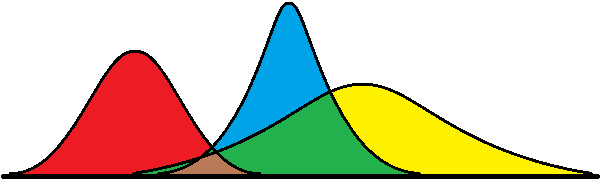
\includegraphics[width=\columnwidth]{GaussianDistOverlap1D.png}}
	}
\caption{The similarity index between three Gaussian distributions is a function the summation measures of overlapping regions of two distributions (green) or three distributions (brown). This concept is easily extended to multivariate distributions.
}\label{fig:SimMeas}
\end{figure}

	
\subsection{Optimal Coalescence Avoidance}

% Explain motivation: minimizing just the uncertainty causes coalescence, so minimizing a similarity index serves to remove coalescence
% Present cost function and the definition of u (from $J_s=\exp(-au)$)
% Derive the remaining terms in a similar fashion to the last paper except with summations where necessary
% Explain which similarities need not be used (when a priori similarity is below some level, the gain of the C-JPDAF is equivalent to that of the MUJPDAF)

Simply minimizing uncertainties of the estimates is well-known to cause coalescence with the JPDAF, but including a similarity index serves to remove this coalescence.
Let $\mathbf{J}\in\Re$ be a cost function of coalescence avoiding filtering as
\begin{align}
\mathbf{J}=J_P+cJ_S,
\end{align}
where $J_P$ is an uncertainty cost that measures the confidence level of the estimates and $J_S$ is a similarity cost that measures a degree of coalescence. The constant $c$ is a positive weighting factor between $J_P$ and $J_S$. 
The estimator gain $K_i$ is selected to minimize the total cost $\mathbf{J}$.
In short, the estimator gain is chosen in the consideration of both uncertainty and coalescence, illustrated in Figure \ref{fig:CostTrends}.


\begin{figure}
\setlength{\unitlength}{0.1\columnwidth}
\centerline{\footnotesize\selectfont
\begin{picture}(8.5,7.3)(-0.5,-0.8)
\put(-0.5,3){\rotatebox{90}{Cost}}
\put(0,0){\includegraphics[width=0.8\columnwidth]{ECC14_fig1.pdf}}
\put(6.2,0.2){\shortstack[c]{Uncertainty\\ cost: $J_P$}}
\put(6.2,2.8){\shortstack[c]{Similarity\\ cost: $J_S$}}
\put(5.7,5.2){\shortstack[c]{Weighted sum:\\ $\mathbf{J}=J_P+cJ_S$}}
\put(4.98,0.78){\circle*{0.1}}
\put(2.48,1.57){\circle*{0.1}}
\put(5.0,-0.3){$K_{MUJPDAF}$}
\put(2.5,-0.3){$K_{C-JPDAF}$}
\put(3.1,-0.8){Estimator gain}
\end{picture}
}
\caption{Illustration of optimal coalescence avoidance: several costs are illustrated with respect to an element of an estimator gain $K$ (red: uncertainty cost $J_P$, blue: similarity cost $J_S$, black: weighted sum). The estimator gain $K_{MUJPDAF}$ is selected to minimize the uncertainty cost. The estimator gain $K_{C-JPDAF}$ is chosen such that the weighted sum of the uncertainty cost and the similarity cost is minimized. In short, at the expense of increased uncertainty at a single step, the proposed approach prevents coalescence. The increased uncertainty at each step is rewarded by reducing the overall estimation error drastically by maintaining correct data association during close proximity missions.}
\label{fig:CostTrends}
\end{figure}

\paragraph*{Uncertainty Cost}
The uncertainty cost $J_P$ is defined as the sum of the trace of each posterior covariance:
\begin{align}
J_P=\sum\limits_{i}\tr{P^+_i},\label{eqn:JP}
\end{align}
where $P^+_{i}$ is obtained by \refeqn{JPDAFCov}.
Therefore, $P_i$ does not depend on $K_j$ for $i\neq j$.
The derivative of $J_P$ is taken from \refeqn{Uncertainty0}
\begin{align}
\label{eqn:CostP}
\frac{\partial J_{P}}{\partial K_{i}}&=2K_iE_i-2(1-\beta_{0,i})P^-_iH_i^T.
\end{align}

\paragraph*{Similarity Cost}
Any shared $z_j$ on estimate $i$ yields an innovation $e_{ij}$.
During the measurement update, this innovation typically has the net effect of drawing the measurement estimate towards $z_j$ if $\beta_{ij}$ is nonzero.
This occurs for all estimates and all measurements; coalescence results when measurement estimates are drawn towards common measurements.
Therefore, coalescence of the JPDAF or MUJPDAF occurs inside the measurement space (e.g. if a sensor provides ranges and bearings, these are in the measurement space as opposed to a Cartesian state vector inside the state space).
Contrary to~\cite{KauLovLee14} where the similarity index is in terms of state space variables, the coalescence avoidance presented in this paper takes place inside the measurement space to most directly remove the coalescence.
Let the posterior measurement estimate be $\hat z_i^+\in\Re^m$ and its innovation be $e_{i}^+\in\Re^m$ that corresponds with its true measurement $z_i\in\Re^m$ (although association is unknown) as
\begin{align}
\hat z_i^+&=H_i\hat x_i^+,
\\
e_{i}^+&=z_i-\hat z_i^+=(H_ix_i+v_i)-H_i\hat x_{i}^+=H_i\tilde x_i^++v_i,
\end{align}
where $\tilde x_i^+=x_i-\hat x_{i}^+$ denotes the error between the true state and the posterior estimate. The posterior innovation covariance $S^+_i\in\Re^{m\times m}$ is given by
\begin{align}
S^+_i&=\mathrm{E}[e_i^+e_i^{+T}]=\mathrm{E}[(H_i\tilde x_i^++v_i)(H_i\tilde x_i^++v_i)^T],\nonumber
\\
&=H_i\mathrm{E}[\tilde x_i^+\tilde x_i^{+T}]H_i^T+\mathrm{E}[vv^T],\nonumber
\\
&=H_iP^+_iH_i^T+R_i.
\end{align}
From these, the similarity cost is defined as
%which are used to define $u_{p q}$ between $\hat z^+_{p}$ and $\hat z^+_{q}$:
\begin{align}
J_S&=\sum\limits_{p,q\in I,p\neq q}\exp (-au_{pq}),
\end{align}
where $u_{pq}\in\Re$ is
\begin{align}
u_{pq} & = (\hat z_{p}^+-\hat z^+_{q})^T{S^+_{pq}}^{-1}(\hat z^+_{p}-\hat z^+_{q})\label{eqn:U},
\end{align}
where $S^+_{pq}=S^+_{p}+S^+_{q}$. \DIFdelbegin %DIFDELCMD < 

%DIFDELCMD < %%%
\DIFdelend Expanding \refeqn{U} with respect to the $p$-th system,
\begin{align}
u_{pq}=&\ 
(H_pK_p{\bf e}_p-\hat z^+_{q})^T
(H_pP^+_{p}H_p^T+R_p+S^+_q)^{-1}\nonumber
\\
&\DIFdelbegin %DIFDELCMD < \ 
%DIFDELCMD < %%%
\DIFdelend \DIFaddbegin \DIFadd{\times  
}\DIFaddend (H_pK_p{\bf e}_p-\hat z^+_{q}).
\end{align}
\newcommand{\Ibd}{\ensuremath{\mathbf{1}_{bd}}}

Next, we find the derivative of the similarity cost as follows.
Let $\Ibd\in \Re^{n\times m}$ be defined such that its $b,d$-th element is one and other elements are zero.
The partial derivative of $u_{pq}$ with respect to the scalar value at the $b,d$-th element of $K_p$, denoted as $K_{p,bd}$, is
\begin{align}
\deriv{u_{pq}}{K_{p,bd}}
=&\ 
(H_p\Ibd{\bf e}_p)^T
{S_{pq}}^{-1}
(H_pK_p{\bf e}_p-\hat z^+_{q})\nonumber
\\
&\ +
(H_pK_p{\bf e}_p-\hat z^+_{q})^T
\mathcal{S}
(H_pK_p{\bf e}_p-\hat z^+_{q})\nonumber
\\
&\ +
(H_pK_p{\bf e}_p-\hat z^+_{q})^T
{S_{pq}}^{-1}
(H_p\Ibd{\bf e}_p),\nonumber
\\
=&\ \{
2(H_p\Ibd{\bf e}_p)^T
{S_{pq}}^{-1} \DIFdelbegin %DIFDELCMD < \nonumber
%DIFDELCMD < \\
%DIFDELCMD < &\ %%%
\DIFdelend +(H_pK_p{\bf e}_p-\hat z^+_{q})^T
\mathcal{S}
\}\DIFaddbegin \nonumber\\
&\DIFadd{\times }\DIFaddend (H_pK_p{\bf e}_p-\hat z^+_{q}),\label{eqn:derivu}
\\
\deriv{u_{pq}}{K_{r,bd}}=&\ 0\quad \mbox{if } r\not\in\{p,q\},\label{eqn:derivu0}
\end{align}
where
\begin{align}
\mathcal{S}=&\ \deriv{{S^+_{pq}}^{-1}}{K_{p,bd}},\nonumber
\\
=&\ {S^+_{pq}}^{-1}
\deriv{\left(H_pP^+_{p}H_p^T+R_p+S^+_q\right)}{K_{p,bd}}
{S^+_{pq}}^{-1},\nonumber
\\
=&\ {S^+_{pq}}^{-1}
H_p
[(1-\beta_{0,p})(\Ibd H_pP_p^-+P_p^-H_p^T\Ibd^T)\nonumber
\\
&\ -\Ibd E_pK_p^T -K_pE_p\Ibd^T]
H_p^T
{S^+_{pq}}^{-1},\label{eqn:SS}
\end{align}
because
\begin{align}
&\deriv{\left(H_pP^+_{p}H_p^T+R_p+S^+_q\right)}{K_{p,bd}}
=
H_p
\deriv{P^+_{p}}{K_{p,bd}}
H_p^T\nonumber
\\
&=
H_p
[(1-\beta_{0,p})(\Ibd H_pP_p^-+P_p^-H_p^T\Ibd^T)\nonumber
\\
&\ \ \ -\Ibd E_pK_p^T -K_pE_p\Ibd^T]
H_p^T.\label{eqn:SSmidpart}
\end{align}
Then, \refeqn{SS} and \refeqn{SSmidpart} are substituted into \refeqn{derivu} or \refeqn{derivu0} to solve
\begin{align}
\label{eqn:JSK}
\deriv{J_S}{K_{p,bd}}=\ -a\sum\limits_{q\in I,q\neq p}\exp (-au_{pq})\deriv{u_{pq}}{K_{p,bd}}.
\end{align}

Necessary conditions for optimality are given by
\begin{align}
\deriv{\mathbf{J}}{K_i} = \deriv{J_P}{K_i} + c \deriv{J_S}{K_i} =0,\label{eqn:NCO}
\end{align}
where $\deriv{J_P}{K_i}$ and $\deriv{J_S}{K_i}$ may be nonzero.
In short, \refeqn{CostP} and \refeqn{JSK} are substituted into \refeqn{NCO} and repeated for all $p$ to obtain the set of optimal gains $\mathcal{K}=\{K_1,K_2,...,K_{n_t}\}$.
Then, the C-JPDAF is completed by updating the state estimate and covariance by using \refeqn{KalEst} and \refeqn{JPDAFCov}, respectively.
As the optimality condition is a nonlinear function of estimator gains, there is no closed-form solution.
Hence, we require a nonlinear equation solver.
When $c=0$, we can show that the optimal gain reduces to that of the MUJPDAF, which is used as an initial guess of numerical solutions.
Therefore, if the number of estimates exhibiting significant similarity is $n_t^*\leq n_t$ and $\mathcal C$ is the number of times \refeqn{NCO} is solved depending on the numerical accuracy, the required iterations is $n_t^*(n_t^*-1)\mathcal C$, where some variables may be reused (e.g. $S^+_{pq}\equiv S^+_{qp}$) and often the effect of \refeqn{derivu} is negligible.






\section{Numerical Examples}
\label{NumRes}

% Two examples with identical realistic (from Vallado book) sensors
% Provide conditions for both scenarios

We consider satellites in the lower earth orbit (LEO) to compare the performances of the conventional JPDAF, the MUJPDAF, and the C-JPDAF.
%The state vector $x=\begin{bmatrix}x_1 & x_2 & x_3 & \dot x_1 & \dot x_2 & \dot x_3\end{bmatrix}^T$ is defined in terms of Cartesian coordinates such that $(x_1,x_2,x_3)$ align with the first three axes of the earth-centered inertial (ECI) frame, where positions are in km and velocities are in km/sec.
%Two-body motion is considered so that for $\vec r=\begin{bmatrix}x_1 & x_2 & x_3\end{bmatrix}^T$, so the nonlinear equations of motion are
Let $\vec r=\begin{bmatrix}x_1 & x_2 & x_3\end{bmatrix}^T$ be the position vector of the $i$-th satellite represented with respect to the Earth-Centered Inertial (ECI) frame.
The equation of motion corresponding to the two-body problem is given by
\begin{align}
\ddot{\vec r}&=-\frac{\mu}{r^3}\vec r=-\mu(\vec r^T\vec r)^{-\frac32}\vec r,
\end{align}
where $\mu=398,600\ \frac{km^3}{sec^2}$ is the gravitational constant of the earth if position is estimated in kilometers and time is measured in seconds~\cite{Val01}.

Let $\delta$ denote an infinitesimal change of a state variable.
The linearized equations of state variable $\vec x=\begin{bmatrix}\vec r & \dot{\vec r}\end{bmatrix}^T\in\Re^6$ are given by
\begin{align}
\begin{bmatrix}
\delta\dot{\vec r} \\ \delta\ddot{\vec r}
\end{bmatrix}
%\delta\dot{\vec x}
=
\begin{bmatrix}
0_{3\times3} & I_{3\times3} \\
\mu\left[3\vec r({\vec r}^T\vec r)^{-\frac52}{\vec r}^T-({\vec r}^T\vec r)^{-\frac32}I_{3\times3}\right] & 0_{3\times3}
\end{bmatrix}
\begin{bmatrix}
\delta\vec r \\ \delta\dot{\vec r}
\end{bmatrix}
%\delta\vec x
.
\end{align}
Defining the above square matrix as $A_{lin}$, the linearized state transition matrix over the time step $dt$ is defined as
\begin{align}
F=\expm{(A_{lin}dt)}
\end{align}
where $\expm$ denotes the matrix exponential function.
%The discretized linearized equations of motion from step $k-1$ to step $k$ are
%\begin{align}
%x_{k}=F_{k-1}x_{k-1}.
%\end{align} 
The process uncertainty may be subject to a variety of perturbations beyond two-body forces, and the process covariance is chosen as $Q=\diag[10^{-6}I_{3\times3}, 10^{-8}I_{3\times3}]$.

The satellites are measured with a single phased-array radar; the measurement space consists of the range $\rho$ between the sensor and the satellite (km), the range rate $\dot\rho$ (km/sec), and topocentric right ascension $\alpha$ and declination $\delta$ (rad) as defined in~\cite{Val01}.
The standard deviations $\sigma_\rho$, $\sigma_\alpha$, and $\sigma_\delta$ are based on the Mahe Ground Station uncertainty data from~\cite{VerSauSco04} and $\sigma_{\dot\rho}$ is taken from~\cite{KurAriAriEfe10}. The measurement uncertainty is $R=\diag[\sigma_\rho^2, \sigma_{\dot\rho}^2, \sigma_\alpha^2, \sigma_\delta^2]=\diag[0.15^2, 0.005^2, (\frac{0.01\pi}{180})^2, (\frac{0.01\pi}{180})^2]$. There is also a $10\%$ chance that a measurement is either deleted or an extraneous measurement is added at each time step.

The conventional JPDAF, MUJPDAF, and C-JPDAF have all been tested with a wide range of objects inside the sensor field of view.
However, this paper focuses on the uncertainty and coalescence of objects in close proximity, so only two or three objects are considered at a time.

%If these objects are not in close proximity with the tracks of interest in the following section, these objects are omitted from the results of this paper because they have an insignificant effect on the tracks of interest.
\paragraph*{Scenario A: Satellites in close proximity pass over a sensor field of view}
The first example compares the JPDAF with the MUJPDAF for tracking two nearby satellites passing over the sensor field of view. The initial conditions of the first two orbits are chosen as
\begin{align}
x_{1,A} & =x_{ref,A}+x_{pert,A}, \quad x_{2,A}=x_{ref,A}-x_{pert,A},\nonumber
\\
x_{ref,A} & =\begin{bmatrix}7000 & 0 & 1000 & 0 & 7.546 & 0\end{bmatrix}^T,\nonumber
\\
 x_{pert,A} & =\begin{bmatrix}
0.2 & 0 & 0 & 0 & -0.105 & 0
\end{bmatrix}^T.
\end{align}
%and the initial conditions of the remaining six orbits are defined as
%\begin{align}
%x_b=x_{ref}+\begin{bmatrix}
%3\times10^{-4}\mathcal{R}_{1,3}, & 10^{-6}\mathcal{R}_{1,3}
%\end{bmatrix}\ \forall \ 2\leq b \leq 8,
%\end{align}
%where $\mathcal{R}_{1,3}$ is a $1\times3$ vector of Gaussian random numbers with mean $0$ and standard deviation $1$ defined by the MATLAB \emph{randn} command.
Two cases are considered with different initial covariances matrices: $P_{0,A1}=10^7\times Q$ for Case A1 and $P_{0,A2}=10^8\times Q$ for Case A2.
These scenarios are chosen because the estimates exhibit large initial uncertainties, so the spread in the innovations term $\tilde P$ from \refeqn{tildeP} affects the updates.
The gain of the MUJPDAF accounts well for $\tilde P$ whereas the gain for the conventional JPDAF does not.
Both data association algorithms are subject to the same set of measurements.
The RMS errors of the position and $J_P$ are summarized in Table \ref{tab:RMSptA}.
The results are plotted in Figure \ref{fig:CompareJPDAFandOJPDAF}.

\DIFaddbegin \DIFadd{ADD A FEW COMMENTS ON THE TABLE AND FIGURES HERE, ESPECIALLY ON TRACK SWAPPING. YOU MAY DELETE THE LAST PARAGRAPH OF THE CONCLUSIONS TO SAVE SPACE.
}

\DIFaddend \begin{table}
\caption{JPDAF and MUJPDAF Comparison: Scenario A}\label{tab:RMSptA}
\centerline{
\begin{tabular}{cccc}\hline
Case & Method & Radial RMS Error (km) & Mean $J_P$\\\hline
\vspace*{-0.02\columnwidth}\\
A1 & JPDAF &  0.12024 & 0.51254\\
A1 & MUJPDAF & 0.10641 & 0.49055\\\hline
\vspace*{-0.02\columnwidth}\\
A2 & JPDAF & 2.6353 & 5.7157\\
A2 & MUJPDAF & 0.19554 & 4.8456\\\hline
\end{tabular}}
\end{table}

\begin{figure}
{
\hspace*{0.05\columnwidth}
\centerline{
	\subfigure[\;Case A1 Orbital Radii]
		{\hspace*{-0.1\columnwidth}\includegraphics[width=0.5\columnwidth]{CaseA1_rad.pdf}}
	\subfigure[\;Case A1 Uncertainty Cost]
		{\hspace*{-0.0\columnwidth}\includegraphics[width=0.5\columnwidth]{CaseA1_Jp.pdf}}
	}
}
{
\hspace*{0.05\columnwidth}
\centerline{
	\subfigure[\;Case A2 Orbital Radii]
		{\hspace*{-0.1\columnwidth}\includegraphics[width=0.5\columnwidth]{CaseA2_rad.pdf}}
	\subfigure[\;Case A2 Uncertainty Cost]
		{\hspace*{-0.0\columnwidth}\includegraphics[width=0.5\columnwidth]{CaseA2_Jp.pdf}}
	}
}
\caption{The orbital radii and uncertainty costs are compared among the algorithms (JPDAF is dashed, MUJPDAF is solid).
These examples show that the posterior uncertainty of the MUJPDAF decreases faster than that of the JPDAF.
The MUJPDAF shares measurement updates less, thereby decreasing coalescence, shown in both Cases A1 and A2.
In Case A2 with the JPDAF, the coalescence causes consistent incorrect associations among the objects, known as track swapping.
}\label{fig:CompareJPDAFandOJPDAF}
\end{figure}

\paragraph*{Scenario B: Three satellites in close proximity have identical initial velocities}
The JPDAF, MUJPDAF, and C-JPDAF algorithms are compared for three satellites with initial conditions
\begin{align}
x_{1,B}&=x_{ref,B}+x_{pert,B}, \quad x_{2,B}=x_{ref,B}-x_{pert,B},
\nonumber\\
x_{3,B}&=x_{ref,B},
\nonumber\\
x_{ref,B}&=\begin{bmatrix}7000 & 0 & 0 & 0 & 7.546 & 0\end{bmatrix}^T,
\nonumber\\
x_{pert,B}&=\begin{bmatrix}
0.025 & 0 & 0 & 0 & 0 & 0
\end{bmatrix}^T,
\end{align}
where $P_{0,B}=Q$.
For the C-JPDAF, the parameters $a=5\times10^{-1}$ and $c=2.3\times10^{-4}$ are used.
The computation time is compared when the algorithms run on a conventional desktop computer.
Given the same measurement set, the results are shown in Table \ref{tab:RMSptB} and Figure \ref{fig:CompareJPDAFandOJPDAFandCJPDAF}.


	% Show coalescence with the JPDAF and MUJPDAF, but avoidance with the C-JPDAF
	% Compare the covariance costs and the computation time


\begin{table}
\caption{JPDAF, MUJPDAF, and C-JPDAF Comparison: Scenario B}\label{tab:RMSptB}
\centerline{
\begin{tabular}{ccc}\hline
Method & Radial RMS Error (km) & Computation time (sec)\\\hline
\vspace*{-0.02\columnwidth}\\
JPDAF & 0.14904 &  1.729\\
MUJPDAF & 0.09935 & 1.725\\
C-JPDAF & 0.046411 & 104.605\\\hline
\end{tabular}
}
\vspace*{-0.08\columnwidth}
\end{table}


\begin{figure}
\centerline{
	\subfigure[\;JPDAF]
		{\includegraphics[width=1\columnwidth]{JPDAF_2000sectest.pdf}}
	}
\centerline{
	\subfigure[\;MUJPDAF]
		{\includegraphics[width=1\columnwidth]{OJPDAF_2000sectest.pdf}}
	}
\centerline{
	\subfigure[\;C-JPDAF]
		{\includegraphics[width=1\columnwidth]{CJPDAF_2000sectest.pdf}}
	}
\caption{The true orbital radii (dashed) and their estimates (solid) for three tracks (blue, black, and red) are compared among all algorithms in Scenario B.
The JPDAF experiences the most coalescence such that the the estimates are not well distinguishable.
The estimates of the MUJPDAF have less uncertainty and therefore less similarity and coalescence.
The C-JPDAF greatly reduces the coalescence, even when measurement are heavily shared, at the cost of increased uncertainty.
}\label{fig:CompareJPDAFandOJPDAFandCJPDAF}
\end{figure}


\section{Conclusions}
\label{Conclusion}

The conventional JPDAF is a well-known algorithm with various applications in data association.
The soft decision approach makes the algorithm robust to missed detections and other clutter.
This paper enhances the JPDAF in two different ways.
First, the JPDAF suffers from a suboptimal Kalman gain.
A minimum uncertainty JPDAF (MUJPDAF) is derived with a new gain that minimizes the full posterior uncertainty.
This gain is computationally comparable to the JPDAF, and shows superior performance in decreasing the estimate uncertainties when the spread in the innovations is nonzero.

Second, both the JPDAF and the MUJPDAF involve measurement sharing, which tends to coalesce estimates in close proximity.
The work from~\cite{KauLovLee14} of the C-JPDAF involves a similarity cost when choosing the estimator gains.
In this paper, the research is matured; the C-JPDAF is generalized for any number of estimates and measurements and the similarity cost is found inside the measurement space where coalescence occurs.
When using the C-JPDAF, there must be a trade-off between uncertainty increase and coalescence removal and powerful computational resources are also required.



%There are several benefits to choosing non-Kalman gains. The Kalman gain is suboptimal with respect to minimizing the linearized a posteriori covariance of the JPDAF. This issue is resolved with using the MUJPDAF, which is computationally comparable and is shown to consistently exhibit less RMS position error and state estimate uncertainty from simulations. The only drawback is that there exists a singularity, which is shown to be easily avoidable and has negligible effect on the filter performance.
%
%However, both the JPDAF and MUJPDAF suffer from coalescence when estimates are in close proximity. The C-JPDAF is derived in a more general sense (same assumptions as the JPDAF and MUJPDAF), which minimizes a weighted cost of state estimate uncertainty and a similarity index of the cluster of any number of estimates. By choosing this index inside the measurement space, the coalescence is more directly removed than prior work in~\cite{KauLovLee14}. To remove coalescence this way, there must be a trade-off between uncertainty increase and coalescence removal and powerful computational resources are also required.

Future work may take two directions: first, the computational requirements of the C-JPDAF make the algorithm infeasible in many scenarios; hence a suboptimal analytic solution that still removes coalescence would make the algorithm suitable for more applications. Second, all three algorithms may undergo further Monte Carlo simulations to show their performance in a variety of scenarios and applications.
These simulations may also serve as direct methods to find the weighting parameters of the C-JPDAF.

% Future work
	% Finding a suboptimal analytic solution to the C-JPDAF to lower the computational requirements
	% Running Monte Carlo simulations on both algorithms to show their performance in a variety of scenarios and applications
	% These simulations may serve as direct methods to find the weighting parameters of the C-JPDAF

\begin{appendix}
\label{append}

\subsection{Invertibility of the new $E_i$} \label{NewPartOfEIsPSD}
Consider that object $i$ is not measured (probability $\beta_{0,i}$), then this portion of the innovation update $e_0=0_{m\times1}$ because no innovation exists where measurements are not available.
Then for all innovations in the set $J^*=\{0\}\cup J$, the Total Probability Theorem holds true for object $i$:
\begin{align}
\sum\limits_{j^*\in J^*}\beta_{ij^*}=1.
\end{align}
From~\cite[Eq. 1.4.16-(1-10)]{ShaRonThi2001}, the covariance spread in the means term of the mixture of $e$ is defined as (note that ${\bf e}_{i}$ remains unchanged)
\begin{align}
\tilde P_e=\sum\limits_{j^*}\beta_{ij^*}(e_{ij^*}-{\bf e}_{i})(e_{ij^*}-{\bf e}_{i})^T,
\end{align}
which is positive semi-definite. Manipulating this equation,
\begin{align}
\tilde P_e=&\sum\limits_{j^*}\beta_{ij^*}e_{ij^*}e_{ij^*}^T
-\sum\limits_{j^*}\beta_{ij^*}e_{ij^*}{\bf e}_{i}^T\nonumber
\\
&
-{\bf e}_{i}\sum\limits_{j^*}\beta_{ij^*}e_{ij^*}^T
+{\bf e}_{i}{\bf e}_{i}^T\nonumber
\\
=&\sum\limits_{j^*}\beta_{ij^*}e_{ij^*}e_{ij^*}^T-{\bf e}_{i}{\bf e}_{i}^T\nonumber
\\
=&\sum\limits_{j}\beta_{ij}e_{ij}e_{ij}^T-{\bf e}_{i}{\bf e}_{i}^T\geq0,
\label{eqn:CovSpreadPSD}
\end{align}
because $e_{i0}\equiv0$. Therefore $E_i$ is invertible $\forall\ 0\leq\beta_{0,i}<1$.


\subsection{The singularity of $E$ is not an infinite limit}
Consider the singularity when $E_i=0$ when no association is made to a track, or equivalently when $\beta^*=(1-\beta_{0,i})=\sum\limits_{j}\beta_j=0$.
It is clear from \refeqn{KalEst} and \refeqn{CovExpanded} that the updates are independent of $K_i$ exactly at this singularity.
We show that $K_i$ is \emph{not} growing without bound nearby this singularity, shown by evaluating the limit at this singularity to ensure boundedness.
Note that if $\sum\limits_{j}\beta_j\rightarrow0\Rightarrow \beta_j\rightarrow0\ \forall\ j$ because of the bounds $\sum\limits_{j}\beta_j\geq\beta_j\geq0\ \forall \ j$.
For clarity, let $\tilde\beta_p=\sum\limits_{j,j\neq p}\beta_j/\sum\limits_{j}\beta_j$ and drop the subscript $i$ because this analysis focuses on a single track.

First, we factor $\beta^*$ from $\sum\limits_{j} \beta_{j}e_{j}e_{j}^T$,
\begin{align}
\sum\limits_{j} \beta_{j}e_{j}e_{j}^T&=(\beta_1e_1e_1^T+\beta_2e_2e_2^T+\DIFdelbegin \DIFdel{...}\DIFdelend \DIFaddbegin \DIFadd{\cdots}\DIFaddend ),\nonumber
\\
&=\beta^*
(e_1e_1^T-\tilde\beta_1e_1e_1^T+
e_2e_2^T-\tilde\beta_2e_2e_2^T+\DIFdelbegin \DIFdel{...}\DIFdelend \DIFaddbegin \DIFadd{\cdots}\DIFaddend ),\nonumber
\\
&=\beta^*(\sum\limits_{j}e_{j}e_{j}^T-\sum\limits_{j}\tilde\beta_je_{j}e_{j}^T).
\end{align}
Similarly, we factor $\beta^*$ from ${{\bf{e}}}{\bf{e}}^T$,
\begin{align}
{{\bf{e}}}{\bf{e}}^T&=\sum\limits_{j} \beta_{j}e_{j}\sum\limits_{j} \beta_{j}e_{j}^T,\nonumber
\\
&=
(\beta_1e_1\sum\limits_{j} \beta_{j}e_{j}^T+\beta_2e_2\sum\limits_{j} \beta_{j}e_{j}^T+\DIFdelbegin \DIFdel{...}\DIFdelend \DIFaddbegin \DIFadd{\cdots}\DIFaddend ),\nonumber
\\
&=\beta^*(e_1\sum\limits_{j} \beta_{j}e_{j}^T-\tilde\beta_1e_1\sum\limits_{j} \beta_{j}e_{j}^T\nonumber
\\
&\ \ \ +e_2\sum\limits_{j} \beta_{j}e_{j}^T-\tilde\beta_2e_2\sum\limits_{j} \beta_{j}e_{j}^T+\DIFdelbegin \DIFdel{...}\DIFdelend \DIFaddbegin \DIFadd{\cdots}\DIFaddend ),\nonumber
\\
&=\beta^*(\sum\limits_{j}e_{j}\sum\limits_{j}\beta_je_{j}^T-\sum\limits_{j}\tilde\beta_je_{j}\sum\limits_{j}\beta_je_{j}^T).
\end{align}
Now that the summations inside $E$ are evaluated, their effects on $K$ are analyzed,
\begin{align}
\lim_{\beta^* \to 0}K&=\lim_{\beta^* \to 0}\beta^*P^-H^T
(\beta^*[S+\sum\limits_{j}e_{j}e_{j}^T\nonumber
\\
&\ \ \ -\sum\limits_{j}\tilde\beta_je_{j}e_{j}^T
-\sum\limits_{j}e_{j}\sum\limits_{j}\beta_je_{j}^T\nonumber
\\
&\ \ \ +\sum\limits_{j}\tilde\beta_je_{j}\sum\limits_{j}\beta_je_{j}^T])^{-1},\nonumber
\\
&=P^-H^T\lim_{\beta^* \to 0}
(S+\sum\limits_{j}e_{j}e_{j}^T-\sum\limits_{j}\tilde\beta_je_{j}e_{j}^T\nonumber
\\
&\ \ \ -\sum\limits_{j}e_{j}\sum\limits_{j}\beta_je_{j}^T+\sum\limits_{j}\tilde\beta_je_{j}\sum\limits_{j}\beta_je_{j}^T)^{-1},
\label{eqn:OptGainNoSingularity}
\end{align}
which not an infinite limit because
\begin{align}
\lim_{\beta^* \to 0}\tilde\beta_p&=\lim_{\beta^* \to 0}\frac{...+\beta_{p-1}+0+\beta_{p+1}+...}{...+\beta_{p-1}+\beta_p+\beta_{p+1}+...}\ \forall\ p\in J,\nonumber
\\
&=1-\lim_{\beta^* \to 0}\frac{\beta_p}{\beta^*},
\end{align}
and therefore the following inequalities hold:
\begin{align}
&0\leq\beta_p\leq\beta^*\leq1\Rightarrow0\leq\lim_{\beta^* \to 0}\frac{\beta_p}{\beta^*}\leq1\Rightarrow0\leq\lim_{\beta^* \to 0}\tilde\beta_p\leq1,
\end{align}
and therefore \refeqn{OptGainNoSingularity} may be solved
\begin{align}
\lim_{\beta^* \to 0}K
%&=
%P^-H^T
%\left(S+\sum\limits_{j}e_{j}e_{j}^T-\sum\limits_{j}{B_j}e_{j}e_{j}^T\right)^{-1}
%\\
&=P^-H^T
(S+\sum\limits_{j}(1-B_j)e_{j}e_{j}^T)^{-1},
\label{eqn:OptGainNoSingularitySolved}
\end{align}
for $0\leq B_j\leq1\ \forall\ j$ and it can be easily seen that the sum of the terms inside the parentheses are invertible.
% and we know that $S+\sum\limits_{j}e_{j}e_{j}^T-\sum\limits_{j}{B_j}e_{j}e_{j}^T$ is invertible because $S$ is positive definite and the remaining terms are a simplified form of \refeqn{CovSpreadPSD}.
From a computational standpoint, for every $\beta^*_i\approx0$, the effect of the measurement update should be negligible, so we may choose $K_i=0_{n\times m}$ near this singularity as it will have little effect on the filter performance; this typically occurs when the object is not measured.
 Choosing this $K_i$ results in no difference between the \DIFdelbegin \DIFdel{a priori and a }\DIFdelend \DIFaddbegin \DIFadd{priori and }\DIFaddend posteriori update results. 

\subsection{The optimal gain and Kalman gain are not guaranteed to be equivalent}
The Kalman gain $K_{Kalman}$ and the MUJPDAF gain $K_{MUJPDAF}$ are not always equivalent with a proof by contradiction. Consider that these gains are equivalent (object subscript $i$ is omitted for clarity):
\begin{align}
&K_{Kalman}=K_{MUJPDAF},\nonumber
\\
%&P^-H^TS^{-1}=(1-\beta_{0})P^-H^TE^{-1},
%\\
&P^-H^TS^{-1}E=(1-\beta_{0})P^-H^T,\nonumber
\\
%&=P^-H^TS^{-1}\left((1-\beta_{0})S+{\sum\limits_{j} \beta_{j}e_{j}e_{j}^T-{\bf{e}}}{\bf{e}}^T\right)
%\\
&=(1-\beta_{0})P^-H^T+P^-H^TS^{-1}({\sum\limits_{j} \beta_{j}e_{j}e_{j}^T-{\bf{e}}}{\bf{e}}^T).\label{eqn:KalMUareSame}
\end{align}
Therefore if \refeqn{KalMUareSame} is true, then
\begin{align}
K_{Kalman}({\sum\limits_{j} \beta_{j}e_{j}e_{j}^T-{\bf{e}}}{\bf{e}}^T)=0,\label{eqn:ContradictionResult}
\end{align}
which implies that the spread in the innovations $\tilde P\equiv0$, not assumed in the JPDAF.
The result of \refeqn{ContradictionResult} may only occur if $K_{Kalman}=0$, the probabilities that each measurement $j$ belongs to each object $i$ are exactly $0$ or $1$, or $K_{Kalman}\perp({\sum\limits_{j} \beta_{j}e_{j}e_{j}^T-{\bf{e}}}{\bf{e}}^T)$ . None of these conditions are \DIFdelbegin \DIFdel{guaranteed}\DIFdelend \DIFaddbegin \DIFadd{satisfied in general}\DIFaddend , so it follows that \DIFdelbegin \DIFdel{$K_{MUJPDAF}=K_{Kalman}$ is not guaranteed}\DIFdelend \DIFaddbegin \DIFadd{the Kalman gain is different from the optimal gain proposed in this paper}\DIFaddend .

\end{appendix}


\bibliography{BibMaster}
\bibliographystyle{IEEEtran}



\end{document}


%\section{Numerical Examples}
%\label{NumRes}
%
%We consider estimation of two satellites in a low-Earth orbit with crossing orbital trajectories. It is assumed that the range toward satellites are measured with unknown origination. 
%
%The dynamics of each satellite is modeled as a two-body problem between each satellite and Earth, i.e., the equations of motion for each orbit only involve force caused by the gravity between the Earth and the satellite and neglect all other forces. For simplicity, both orbits occupy the same plane, so polar coordinates are used to define our state variable $x=\begin{bmatrix} r & \dot r & \theta & \dot \theta\end{bmatrix}^{T}$. The resulting equations of motion of each satellite are given by
%\begin{gather*}
%\ddot r - r\dot\theta^2 = -\frac{\mu}{r^2},\\
%r\ddot\theta + 2\dot r\dot\theta =0,
%\end{gather*}
%where $\mu=3.986\times10^5\, \mathrm{km^3/s^2}$ is the gravitational parameter of the Earth. These are linearized to obtain the system matrix of the discrete-time linear equations of motion considered in this paper:
%\begin{align}
%A_{i_k}=
%\exp\left(\begin{bmatrix}
%0 & 1 & 0 & 0 \\
%\frac{2\mu}{r_{i_k}^3} +\dot\theta^2_{i_k} & 0 & 0 & 2r_{i_k}\dot \theta_{i_k} \\
%0 & 0 & 0 & 1 \\
%2r_{i_k}^{-2}\dot r_{i_k}\dot\theta_{i_k} & -2r^{-1}\dot\theta_{i_k} & 0 &  -2r_{i_k}^{-1}\dot r_{i_k}\\
%\end{bmatrix}\Delta t\right).
%\end{align}
%%where  and $H=\begin{bmatrix} 1 & 0 & 0 & 0\end{bmatrix}$.
%
%
%The initial estimates of the states are designed to occur shortly before the two trajectories cross paths near $r_{ref}=7000km$ from the center of the earth; for the time to complete a circular orbit at this radius, $t_{ref}=2\pi \sqrt{\frac{r_{ref}^3}{\mu}}$, we can solve for a reference circular orbit $X_{ref}=\begin{bmatrix} r_{ref} & 0 & 0 & \frac{2\pi}{t_{ref}}\end{bmatrix}^T$, then perturb this orbit slightly by $X_{pert}=\begin{bmatrix} 0.40 & 0 & 0 & -1.5\times10^{-5}\end{bmatrix}^T$. We can easily choose the initial conditions to be $X_{1_0}= X_{ref}+X_{pert}$ and $X_{2_0}= X_{ref}-X_{pert}$. The initial estimates are assumed to be relatively accurate: there is no need to simulate large uncertainty when the paths are initially sufficiently far apart because this paper is concerned with the coalescence when the objects are close together, so the state and covariance will have been determined by simulated measurements while the estimates were still spread significantly apart; hence for both estimates, the initial covariance was chosen to be $P_0=diag(\begin{bmatrix}
%2.5\times10^{-4} & 2.5\times10^{-6} & 3.9\times10^{-8} & 3.9\times10^{-8} \end{bmatrix})$.
%The process noise was chosen to be equivalent for both estimates such that $Q=diag(\begin{bmatrix}
%2.5\times10^{-5} & 2.5\times10^{-7} & 3.9\times10^{-9}& 3.9\times10^{-9}\end{bmatrix})$ and $R=\begin{bmatrix}
%2.25\times10^{-2}
%\end{bmatrix}$ applied at each time step.
%
%%\EditTL{Put the values of $P_0$, $Q$ and $R$ here. Describe how the measurements are switched between two satellites. }
%
%
%Three filtering approaches are applied, namely extended Kalman filter (EKF), JPDAF, and C-JPDAF. For the EKF, it is assumed that the correct measurement origination is know with certainty, i.e., all of the measurements are associated to the correct object. This serves as an ideal reference case to be compared with JPDAF and C-JPDAF. For the C-JPDAF, the weighting parameters of the cost are chosen as $a=0.02$ and $c=5\times10^{-5}$. We propagate the nonlinear equations of motion numerically using Matlab, and we generate a measurement at every $0.1$ seconds with an equal likelihood that its origination is from either object such that all three algorithms are subject to identical noisy measurements. The estimates are propagated with their nonlinear equations of motion; the data association and filtering algorithms use the linearized form.
%
%\begin{figure}
%\centerline{
%	\subfigure[EKF]{\hspace*{0.07\textwidth}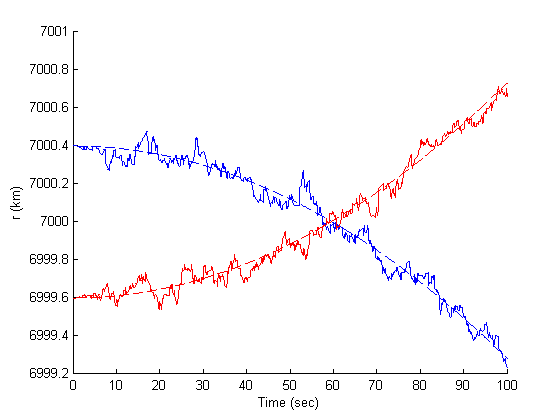
\includegraphics[width=9cm]{EKF.png}\hspace*{0.07\textwidth}}
%	}
%\centerline{
%	\subfigure[JPDAF]{\hspace*{0.07\textwidth}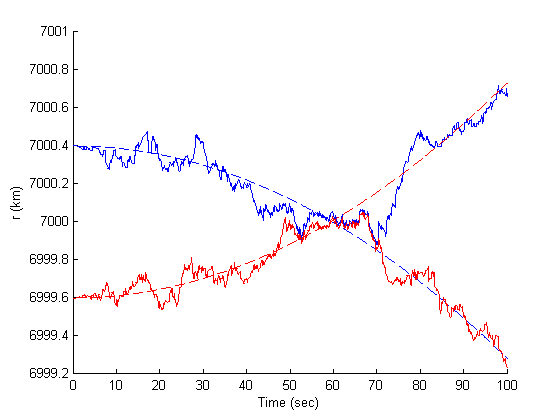
\includegraphics[width=9cm]{JPDAF.png}\hspace*{0.07\textwidth}}
%	}
%\centerline{
%	\subfigure[C-JPDAF]{\hspace*{0.07\textwidth}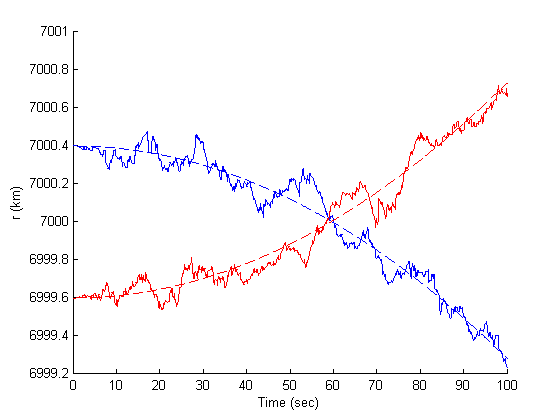
\includegraphics[width=9cm]{CAOJPDAF.png}\hspace*{0.05\textwidth}}
%	}
%\caption{Object 1 is represented in blue and object 2 is represented in red. A solid line represents an estimate and a dotted line represents the truth. The JPDAF is subject to coalescence of the neighboring track, causing the estimations to switch trajectories. The C-JPDAF is subject to much less coalescence and hence does not exhibit this problem.}
%\label{AllAlgorithms}
%\end{figure}
%
%The corresponding results for each of the EKF, JPDAF, and C-JPDAF algorithms are illustrated in Figure \ref{AllAlgorithms}. 
%First, EKF exhibits good estimation performance as there is no error or uncertainty in data association. The performance of JPDA is similar to EKF when two satellites are far apart from each other. However, when $50\leq t\leq 70$ seconds, two satellites become closer, and the estimated states are coalesced. When $t\geq 70$ seconds, the estimated states are incorrectly crossed. This illustrates undesirable performance of JPDAF especially for crossing objects. 
%
%The proposed C-JPDAF does not exhibit the incorrect, crossed estimation of JPDA, and the estimated states follow each of the correct trajectories throughout the crossing orbital trajectories. The resulting RMS errors for the orbital radius of each method are summarized at Table \ref{tab:RMS}. This illustrates that the performance of the proposed C-JPDAF is comparable to EKF where there is no error in data association. 
%
%\begin{table}
%\caption{Estimation results}\label{tab:RMS}
%\centerline{
%\begin{tabular}{ccc}\hline
%Method & Radial RMS Error (km) & Computation time (sec) \\\hline
%EKF & 1.438e-05 &6.118\\
%JPDAF & 7.1242e-05 &6.130\\
%C-JPDAF & 2.3145e-05  & 19.864 \\\hline
%\end{tabular}}
%\end{table}
%
%The major drawback of the C-JPDAF is the added computation time. However, the results of all three simulated algorithms (EKF, JPDAF, and C-JPDAF) are nearly identical when the estimates are not near the crossing region. Hence, the C-JPDAF can be turned on only during these close proximity regions, then turned off when unnecessary to improve the computational efficiency. 
%
%%_______________________________________________%
%
%\section{Conclusions and Future Work}
%\label{ConclusionFutureWork}
%We explore a new approach to reduce coalescence of close proximity multi-object tracking. The estimator gains are chosen such that a weighted cost with respect to posterior uncertainty and similarity is minimized. The proximity similarity portion of the Matusita's measure is chosen to evaluate the similarity. Necessary conditions for optimality are derived, and they are solved numerically to obtain optimal estimator gains. Numerical examples illustrate that it exhibits excellent estimation and data association properties for crossing tracks in close proximity. Compared with other techniques to avoid coalescence, the proposed approach has simpler structures. Future works include generalizing C-JPDAF for arbitrary number of objects with clutter, and improving the computational efficiencies. 
